\documentclass[english,10pt]{beamer}

\usepackage{amsmath,amssymb,amsthm,bbm}
\usepackage{graphicx,transparent,eso-pic}
\usepackage[document]{ragged2e}
\usepackage{pagecolor,color,ulem,soul}


\usetheme{Warsaw}

\setbeamertemplate{footline}[text line]{}
\setbeamercolor{structure}{fg=purple!50!blue, bg=purple!50!blue}

\setbeamercovered{transparent}

\newcommand{\jframe}[2]{\frame{\frametitle{#1}\justify{#2}}}

\newcommand{\noun}[1]{\textsc{#1}}
\newcommand{\jitem}[1]{\item \begin{justify} #1 \end{justify} \vfill{}}
\newcommand{\sframe}[2]{\frame{\frametitle{#1} #2}}


\begin{document}
\title{Morphogenesis}


\author{}

\date{July 7th 2016}

\begin{frame}
\titlepage
\end{frame}


%%%%%%%%%%%%%%%%%%
%% Presentation outline
%%
%%  - context : simple def ? used in a lot of field. 
%%  - literature, research question and methodology
%%  - history of the notion
%% (Next slides give precise example)
%%  - ex1 : biology1
%%  - ex2 : biology2
%%  - ex3 : urban geography
%%  - ex4 : psychology
%%
%%  - slide with outline of the overall variety
%%
%%   - synthesis of concepts - what in common/what ≠
%%   - proposition of general framework : self-org/morph/autopiesis
%%
%%   - further developments : quantitative epistemo ?
%%
%%   - conclusion
%%
%%



%%%%%%%%%%%%%%%%%%
\section{Introduction}

\jframe{A simple definition ?}{
% introduce the notion, try to give a simple def.

}

\jframe{Research Question}{
% literature on similar approach, research question, methodo

}



\jframe{History of the notion}{

}


%%%%%%%%%%%%%%%%%%
\section{Examples}

\jframe{Example : How do patterns arise during animal development}{
% bio 1

}

\jframe{Example : biology}{
% bio 2 , the most ≠ possible from the first

}


\jframe{Example : urban geography}{

\textit{Simple model of urban morphogenesis in~\cite{raimbault2014hybrid}}

$\rightarrow$ local interactions captured by density feedback
$\rightarrow$ global position captured by network centrality feedback and accessibility to amenities

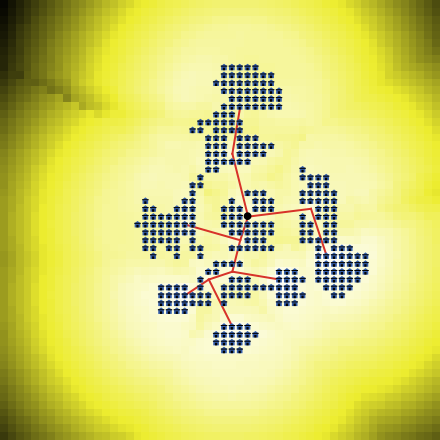
\includegraphics[width=0.5\textwidth]{figures/radiant}
}


\jframe{Example : psychology}{

}


\jframe{Overview}{
% other numerous examples of fields/case of application
\begin{itemize}
\item \textbf{Biology} External phenotype morphogenesis (ant colony)~\cite{minter2012morphogenesis} ; symbiosis of species~\cite{chapman1998morphogenesis}
\item \textbf{Social Sciences} : Archeology~\cite{renfrew1978trajectory}
\item \textbf{Epistemology} : \cite{gilbert2003morphogenesis}
\end{itemize}

}



%%%%%%%%%%%%%%%%%%
\section{Synthesis}


\jframe{Concepts}{
% common points and differences in concepts

}



\jframe{Framework Proposition}{
% Generalisation based on the inclusion Self-organization > morphogenesis > autopoiesis > life.
% seems to include most of fields and ideas ?

% Processes of morphogenesis : local interaction vs information diffusion

}



\jframe{Perspectives}{

}


\jframe{Conclusion}{

}



